\documentclass[tikz, border=10pt]{standalone}
\usepackage[T1]{fontenc}
\usepackage[utf8]{inputenc}
\usepackage{lmodern}
\usepackage[table]{xcolor}
\definecolor{IntelBlue}{HTML}{0068B5}
\definecolor{IntelLightBlue}{HTML}{DDEEF9}
\definecolor{FpgaOrange}{HTML}{E67E22}
\definecolor{FpgaLight}{HTML}{FDEBD0}
\definecolor{HpsGreen}{HTML}{1A7A4A}
\definecolor{HpsLight}{HTML}{D5F5E3}
\definecolor{GrayBg}{HTML}{F2F3F4}
\definecolor{GrayBorder}{HTML}{AAB7B8}
\definecolor{PassGreen}{HTML}{D5F5E3}
\definecolor{PassGreenDark}{HTML}{1E8449}
\definecolor{RowAlt}{HTML}{F7F9FB}
\definecolor{SummaryBg}{HTML}{EBF5FB}
\definecolor{NodeFill}{HTML}{D6EAF8}
\definecolor{NodeBorder}{HTML}{1B4F72}
\definecolor{InitFill}{HTML}{E5E7E9}
\definecolor{InitBorder}{HTML}{717D7E}
\definecolor{SleepFill}{HTML}{FEF5E7}
\definecolor{SleepBorder}{HTML}{935116}
\definecolor{MsgFill}{HTML}{D1F2EB}
\definecolor{MsgBorder}{HTML}{0E6655}
\definecolor{TimeoutRed}{HTML}{C0392B}
\definecolor{BtnBlue}{HTML}{1A5276}
\definecolor{ArrowGray}{HTML}{717D7E}
\usepackage{tikz}
\usetikzlibrary{shapes.geometric, arrows.meta, positioning, fit, backgrounds, calc, decorations.pathreplacing, bending, shadows.blur}
\begin{document}
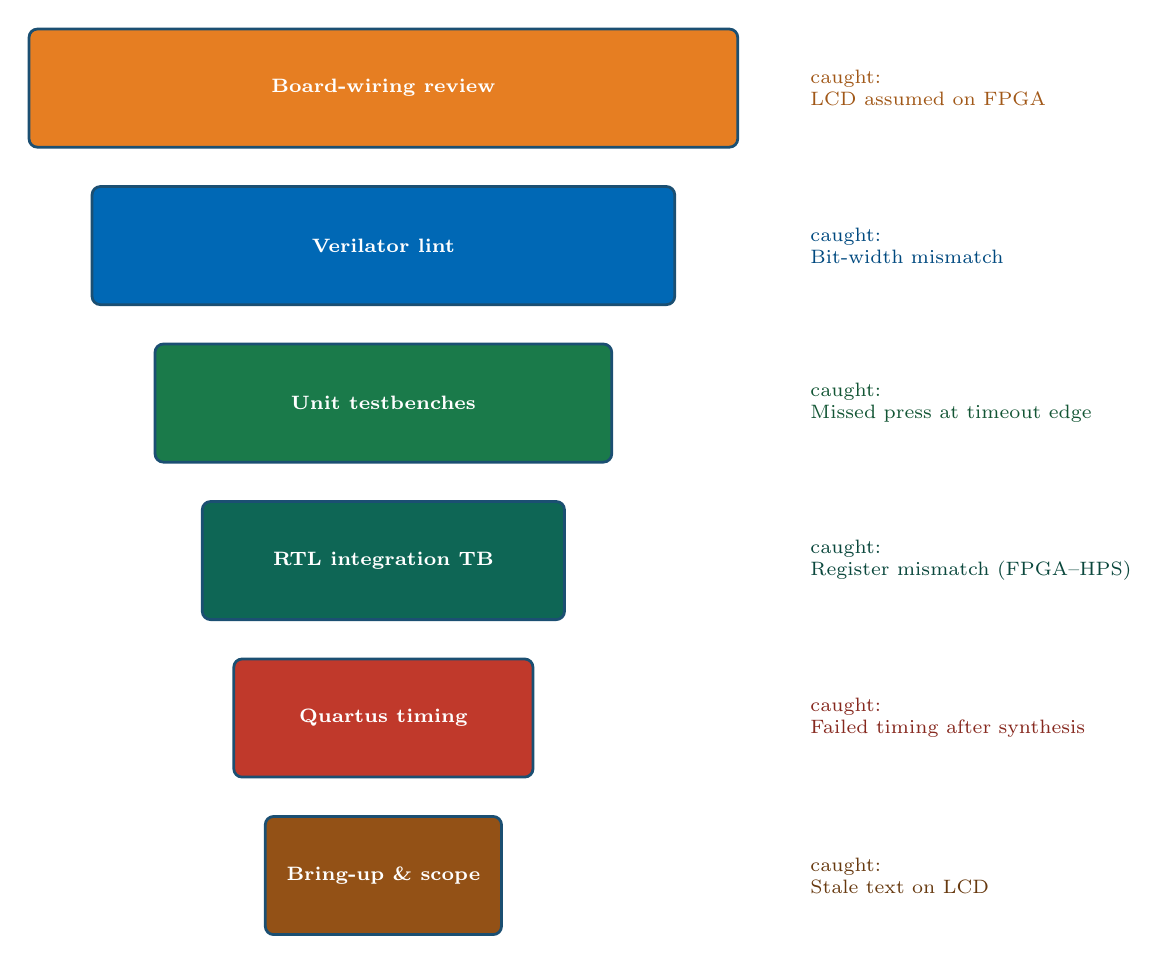
\begin{tikzpicture}[
  gate/.style={rectangle, rounded corners=3pt,
               draw=NodeBorder, line width=1pt, align=center,
               font=\scriptsize\bfseries, text=N2},
  lbl/.style={font=\scriptsize, align=left, anchor=west},
]
% Widths decrease strictly top-to-bottom so the boxes read as a narrowing
% funnel. Labels are kept short enough that none exceeds its box width (a long
% label auto-expands its node and would break the monotonic narrowing); the
% full defect each gate caught is spelled out in the caught: annotation beside
% it, so nothing is lost.
\def\gatewidth{9.0}
\foreach \i/\y/\w/\clr/\gate/\defect in {
  0/0.0/9.0/FpgaOrange/Board-wiring review/LCD assumed on FPGA,
  1/-2.0/7.4/IntelBlue/Verilator lint/Bit-width mismatch,
  2/-4.0/5.8/HpsGreen/Unit testbenches/Missed press at timeout edge,
  3/-6.0/4.6/MsgBorder/RTL integration TB/Register mismatch (FPGA--HPS),
  4/-8.0/3.8/TimeoutRed/Quartus timing/Failed timing after synthesis,
  5/-10.0/3.0/SleepBorder/Bring-up \& scope/Stale text on LCD
} {
  \node[gate, minimum width=\w cm, minimum height=1.5cm,
        fill=\clr, text=white] at (0,\y) {\gate};
  \node[lbl, text=\clr!70!black] at (5.3,\y) {caught:\\\defect};
}
\end{tikzpicture}
\end{document}
